%форматирование размера документа
\documentclass[11pt, a4paper]{article}

\usepackage{geometry}
% total - determines printable width, height
\geometry{ 
	a4paper, total={190mm,267mm}
}

%----text,fonts------------------------------------------------------------------------------------
\usepackage{mmap}
\usepackage[T2A]{fontenc}
\usepackage[utf8]{inputenc}
\usepackage[english, russian]{babel}
\usepackage{setspace}
\setstretch{0,9}
\usepackage{fancyvrb}

%----math,graphics---------------------------------------------------------------------------------
\usepackage{amsmath,amsfonts,amssymb}
\usepackage{amsthm}
\usepackage{listings}
\usepackage{xcolor}
\usepackage{filecontents}
\usepackage{xcolor}
\usepackage{hyperref}

 % Цвета для гиперссылок
\definecolor{linkcolor}{HTML}{799B03} % цвет ссылок
\definecolor{urlcolor}{HTML}{799B03} % цвет гиперссылок

\hypersetup{pdfstartview=FitH,  linkcolor=linkcolor,urlcolor=urlcolor, colorlinks=true}

\usepackage{tikz}
\usetikzlibrary{calc}
\usepackage{pgfplots}
\pgfplotsset{
	compat=1.17
}

\usepackage{graphicx}
\graphicspath{{images/}}
  
\usepackage{wrapfig}
\usepackage{tabularx}

% relative importing
\usepackage{import}

% \input{./language.tex}

\begin{document}

\import{.}{titular.tex}

\newpage

\section{Описание задания}

\begin{enumerate}
    \item Датасет с данными про оценки студентов инженерного и педагогического факультетов (для данного датасета нужно ввести метрику: студент успешный/неуспешный на основании грейда)
    \item Отобрать случайным образом sqrt(n) признаков.
    \item Реализовать без использования сторонних библиотек построение дерева решений (numpy и pandas использовать можно).
    \item Провести оценку реализованного алгоритма с использованием Accuracy, precision и recall
    \item Построить AUC-ROC и AUC-PR.
\end{enumerate}

\section{Реализация.}

\subsection{Подсчет количества признаков}

Общее количество признаков в датасете - 22. Тогда требуемое количество: 

$$
  k = \lceil \sqrt{32} \rceil = 5
$$

\subsection{Реализация и вывод формул}

Обратиться к пункту 3.

\subsection{Оценка реализованного алгоритма с использованием accuracy, precision и recall}

\begin{Verbatim}
Accuracy:  0.8203865566908778
Precision:  0.7729890764647468
Recall:  0.9249049429657795
\end{Verbatim}

\subsection{AUC-ROC и AUC-PR}

\begin{figure}[ht]
  \centering
  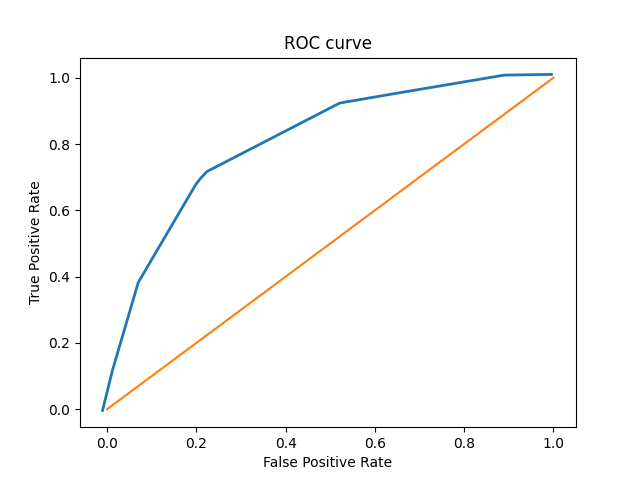
\includegraphics[width=0.7\textwidth]{ROC.png}
  % \label{fig:result-png}
\end{figure}

\newpage

\begin{figure}[ht]
  \centering
  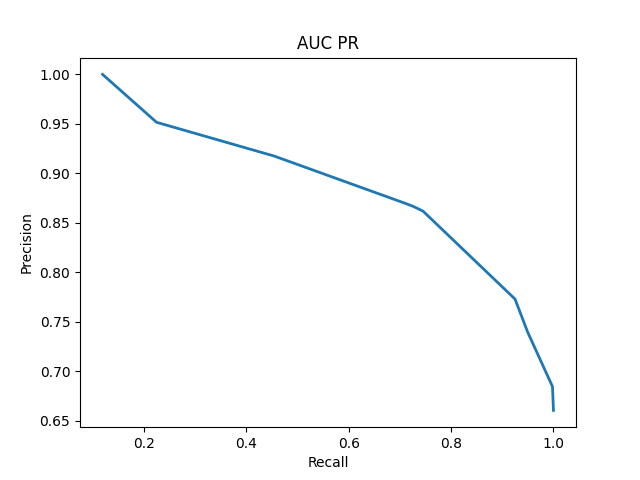
\includegraphics[width=0.7\textwidth]{PR.png}
  % \label{fig:result-png}
\end{figure}

\section{Исходный код}

 \href{https://github.com/dmittrey/Artificial-intelligence-lab3}{https://github.com/dmittrey/Artificial-intelligence-lab3}
 
\section{Вывод.}

\noindent В ходе выполнения лабораторной работы я познакомился с алгоритмом C4.5 и реализовал его на питоне. Также
вспомнил, что такое accuracy, precision, recall, а также разобрался, как строить графики AUC-ROC, AUC-PR.

\end{document}
